\section{Antecedentes}\label{sec:background}

Buscamos desplegar aplicaciones de streaming video understanding (SVU)~\cite{zhang2024flashvstream,Shangzhe2025streaming} en entornos con memoria restringida. A diferencia de offline video understanding (OVU)~\cite{MLVU,fu2024videomme,wu2024longvideobench}, que asume acceso al video completo, SVU debe procesar flujos de video arbitrariamente largos y responder preguntas en cualquier instante usando solo los frames observados hasta ese momento. Dado un flujo de video $V_T := [v_1, v_2, \dots, v_T]$ con $T$ frames y un conjunto de preguntas $Q = {q_1, q_2, \dots, q_N}$, SVU responde cada pregunta $q_i$ en el tiempo $t$ ($1 \le t \le T$) usando únicamente los frames observados $V_t := [v_1, v_2, \dots, v_t]$.

Como SVU trabaja con flujos de video no acotados, el procesamiento eficiente en memoria es esencial. En esta sección describimos cómo los multimodal large language models (MLLMs) manejan videos largos, revisamos enfoques previos para reducir memoria en OVU y analizamos sus limitaciones al aplicarlos a SVU. (Véase el Apéndice.~\ref{sec:related} para una discusión detallada del trabajo relacionado.)

\subsection{Preliminar: Offline Long Video Understanding}

\paragraph{Procesamiento de video en MLLMs.} Los Multimodal Large Language Models (MLLMs)~\cite{zhang2024llavanext-video,qwen2.5,Qwen2VL} procesan videos offline mediante una tubería estructurada (Fig.~\ref{fig:background}(a)). Dado un video $V_T := [v_1, v_2, \dots, v_T]$ de $T$ frames muestreados uniformemente, un vision encoder $f_{\text{ViT}}$ transforma cada frame en visual tokens:
\begin{equation}
X = f_{\text{ViT}}(V_T) = [x_1, x_2, \dots, x_N] \in \mathbb{R}^{N \times D},
\label{eq:vision_encoding}
\end{equation}
donde $N = P \times T$ denota el número total de tokens muestreados, donde $P$ es el número de tokens por frame (determinado por la resolución de entrada y el tamaño de patch de ViT), y $D$ es la dimensión del embedding del token.

La secuencia de tokens $X$ se pasa luego al LLM en dos fases: Prefill y Decoding. Durante la fase de Prefill (Fig.~\ref{fig:background}(a), paso 2), todos los tokens se procesan de una vez para construir la KV cache inicial. La operación de atención calcula:
\begin{equation}
Q = XW_q, \quad K = XW_k, \quad V = XW_v, \quad O^{\text{attn}} = \text{Softmax}\left(\frac{QK^\top}{\sqrt{D}} + M\right)V,
\label{eq:attention_combined}
\end{equation}
donde $W_q, W_k, W_v \in \mathbb{R}^{D \times D}$ son matrices de proyección y $M$ es una máscara causal que impone decoding autorregresivo.

En la fase de Decoding (Fig.~\ref{fig:background}(a), paso 3), el modelo genera tokens uno por uno usando keys y values almacenados de la fase de prefill. Para evitar cómputo redundante, la KV cache $\mathcal{C} = (K, V)$ se actualiza de forma incremental:
\begin{equation}
\mathcal{C}_{t+1} = \left(\{K,k_{t+1}\}, \{V,v_{t+1}\}\right),
\label{eq:kv_cache}
\end{equation}
donde $k_{t+1}, v_{t+1}$ corresponden a los embeddings KV del token recién procesado.


\begin{figure*}[t!]
    \centerline{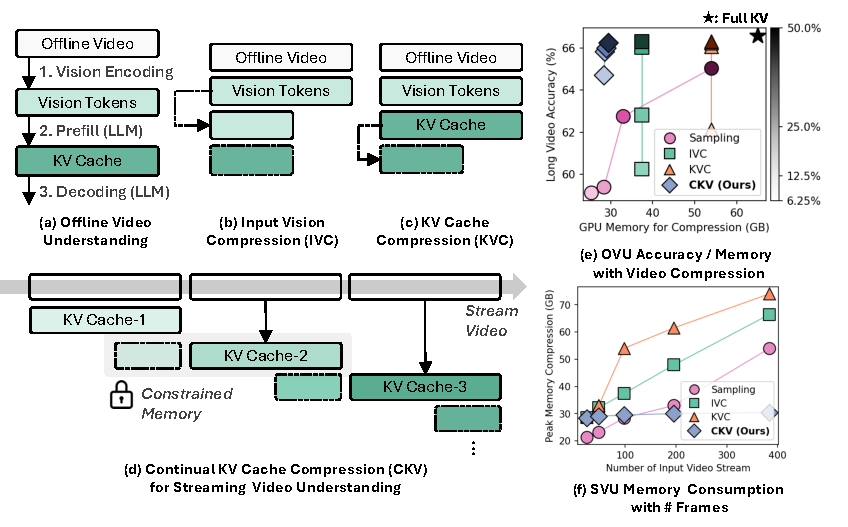
\includegraphics[width=0.95\textwidth]{Figures/fig1.pdf}}\caption{\textbf{Video Understanding y compresión en MLLMs.} (a) tubería OVU; (b) IVC: comprime vision tokens después del encoding; (c) KVC: comprime la KV cache después del prefill; (d) CKV: procesa y comprime iterativamente KV caches para restringir el uso de memoria; (e) Exactitud vs. consumo de memoria GPU para la compresión en cuatro razones de reducción de tokens (50\%, 25\%, 12.5\%, 6.25\%) sobre MLVU usando \texttt{Qwen-2-VL-7B}. LongVU\cite{shen2024longvu} se usa para IVC y SnapKV\cite{li2024snapkv} para KVC; (f) uso de memoria GPU a medida que aumenta la longitud del flujo de video de entrada. IVC/KVC/CKV apuntan a una cache de 6K; Sampling usa 1/4 de los frames de entrada. Medido en una única GPU A100 de 80GB.}
    \vspace{-2mm}
\label{fig:background}

\end{figure*}


\subsection{Estrategias de compresión offline para video largo}
\label{sec:motivation:offline}

Los videos largos producen secuencias de tokens $X$ extremadamente extensas, lo que genera requisitos prohibitivos de memoria GPU y latencia durante el decoding. Trabajos previos abordan este cuello de botella en el entorno offline mediante tres clases de métodos (Fig.~\ref{fig:background}a–c):

\textbf{(1) Frame Sampling~\cite{feichtenhofer2019slowfastnetworksvideorecognition}.}  
Muestrear uniformemente un clip más corto $V'_{T'} \!\subseteq\! V_T$ reduce la longitud de entrada y, en consecuencia, el uso de memoria también se reduce en proporción a la tasa de compresión. %but inevitably discards fine-grained temporal cues and hurts accuracy.

\textbf{(2) Input-Vision Compression (IVC)~\cite{shen2024longvu,tao2024dycokedynamiccompressiontokens}.}  
Después del vision encoding, IVC poda agresivamente los vision tokens redundantes y conserva solo un subconjunto saliente $X' \!\subseteq\! X$ (Fig.~\ref{fig:background}b) para reducir el contexto entregado al language decoder y así realizar un Prefill comprimido en memoria.

\textbf{(3) KV cache Compression (KVC)~\cite{li2024snapkv,fu2024headkv,chen2024image}.}  
Realiza la compresión después del prefill: KVC calcula puntajes de importancia  
$u_t\!=\!\sum_{i=N-w}^{N}\!\text{Attn}(x_i\!\rightarrow\!x_t)$  
sobre los últimos $w$ tokens y conserva las entradas top-$M$ para el presupuesto de memoria $M$ aplicando la política de expulsión $\pi$, produciendo una cache comprimida  
$\mathcal{C}'=\pi(\mathcal{C})$ para un Decoding comprimido en memoria.
(Fig.~\ref{fig:background}c). Nótese que la política de expulsión $\pi$ depende fuertemente del contenido de los últimos $w$ tokens, reflejando la consulta del usuario, y por ello se la denomina método de compresión de cache dependiente de la consulta (véase el Apéndice.~\ref{appn:query_agnostic} para más análisis).

Estas técnicas son efectivas cuando el video completo está disponible de antemano, pero asumen implícitamente (i) memoria no restringida para la compresión y (ii) una consulta conocida o fácilmente aproximable.




\subsection{Desafíos en Streaming Video Understanding}
\label{sec:motivation:streaming}

La Fig.~\ref{fig:background}(e) compara tres métodos de compresión \textit{offline} sobre un video fijo de 50\,K tokens en cuatro razones de compresión (los tonos más oscuros indican razones más altas: 50\%, 25\%, 12.5\%, 6.25\%), revelando un trade-off fundamental entre uso de memoria y exactitud. \textit{Frame sampling} omite frames para ahorrar memoria, pero degrada severamente la exactitud de reconocimiento. Aumentar la tasa de muestreo mejora la exactitud, pero infla rápidamente el uso de memoria. \textit{IVC} comienza con una gran huella de memoria para todos los vision tokens antes de seleccionar cuáles descartar. \textit{KVC}, que opera sobre características key--value más expresivas, logra la mayor exactitud pero requiere la mayor cache de Prefill. Notablemente, incluso bajo un escenario offline favorable---con acceso completo al video y una consulta offline---ninguno de los métodos logra simultáneamente alta exactitud y bajo uso de memoria.

Este trade-off se vuelve más severo en el escenario de streaming video understanding (SVU). Como se muestra en la Fig.\ref{fig:background}(f), el pico de uso de memoria GPU aumenta con la longitud del flujo. KVC exhibe un crecimiento de memoria casi lineal, ya que debe materializar todos los vision tokens y construir la KV cache completa antes de comprimir. Además, debido a su naturaleza dependiente de la consulta, KVC debe \textit{re-ejecutar} la etapa de prefill intensiva en memoria cada vez que cambia la consulta del usuario. Frame sampling e IVC también crecen linealmente, aunque más lentamente, y terminan superando la capacidad de memoria de dispositivos edge prácticos (por ejemplo, 32GB\cite{Karumbunathan2022JetsonAGXOrin}) a medida que el flujo continúa. ReKV~\cite{Shangzhe2025streaming}, un método KVC reciente, aborda esto descargando la KV cache a memoria CPU, pero introduce una sobrecarga considerable de offloading y latencia de compresión. 

Estos hallazgos resaltan dos requisitos centrales para SVU: (1) un presupuesto de memoria fijo que no crezca con la longitud del flujo, y (2) estrategias de retención de tokens independientes de la consulta. Los métodos existentes no cumplen al menos uno de estos requisitos, lo que limita su idoneidad para SVU. 
Para superar esto, proponemos Continual KV cache compression (CKV), ilustrado en la Fig.~\ref{fig:background}(d). CKV procesa frames en bloques pequeños y comprime la cache cada vez que se alcanza el límite fijo de memoria, garantizando un uso constante de memoria durante todo el streaming. Además, para la retención de tokens independiente de la consulta, nuestro enfoque emplea métricas espaciotemporales ligeras para identificar y preservar tokens semánticamente significativos sin depender de consultas futuras. Como resultado, a pesar de operar bajo restricciones estrictas de memoria, CKV logra una exactitud comparable o superior a KVC (Fig.\ref{fig:background}(e)), mientras consume mucha menos memoria que IVC o frame sampling (Fig.~\ref{fig:background}(f)). Los detalles algorítmicos se describen en la Sec.\ref{sec:method}.
